\documentclass[11pt]{article}
\usepackage[T1]{fontenc}
\usepackage[utf8]{inputenc}
\usepackage{graphicx}
\usepackage{minitoc}
\usepackage[french]{babel}
\usepackage[right=2.5cm, bottom=2.5cm,top=2.5cm, left=2.5cm]{geometry}
\title{\vspace{\fill} Interface et Multimédia \\ ~\textbf{IFT-215} \\~\\ Travail Pratique 4}
\author{Amandine Fouillet - 14 130 638 ~\\ Frank Chassing - 14 153 710 ~\\ Laurent Sénécal-Léonard - 14 143 484}
\date{\today \vspace{\fill}}

\begin{document}
\maketitle
\newpage \thispagestyle{empty}
\null
\newpage
\tableofcontents

\newpage
\section*{Introduction \markboth{INTRODUCTION}{}}
\addcontentsline{toc}{section}{Introduction}

\section{Modélisation de la gestion de la Communication}
\begin{figure}[!h]
        \centering 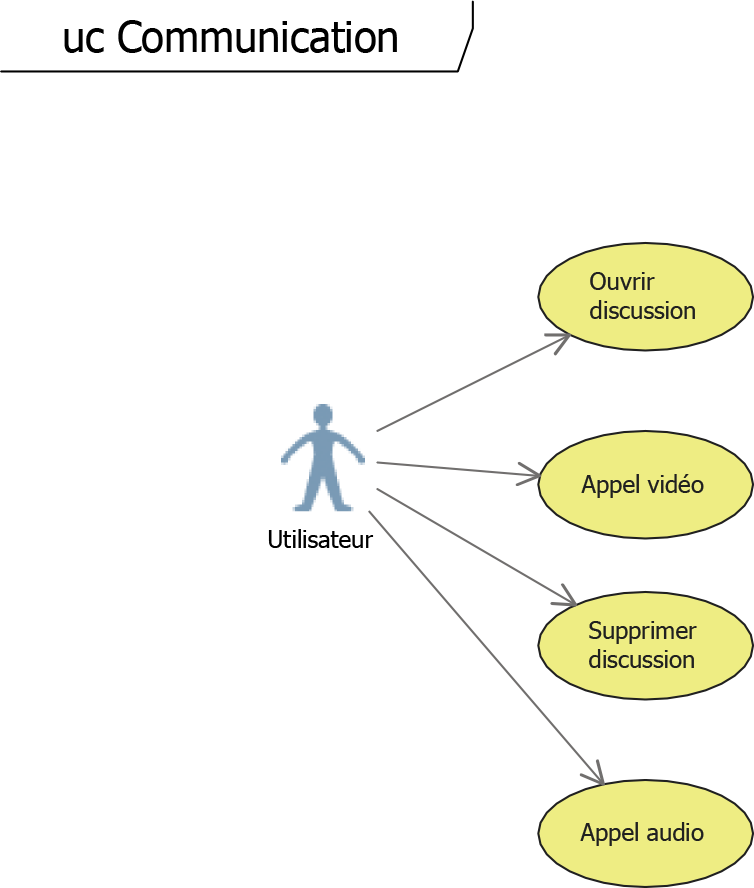
\includegraphics[scale=1]{ucCom.png}
        \caption{Cas d'utilisation communication}
         \label{fig:ucCom}
\end{figure}
\begin{figure}[!h]
        \centering 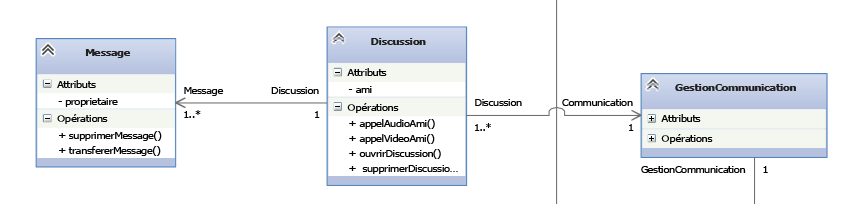
\includegraphics[scale=1]{com.png}
        \caption{Diagramme de classe communication}
         \label{fig:com}
\end{figure}

\newpage
\section{Modélisation de la gestion des Photos}
\begin{figure}[!h]
        \centering 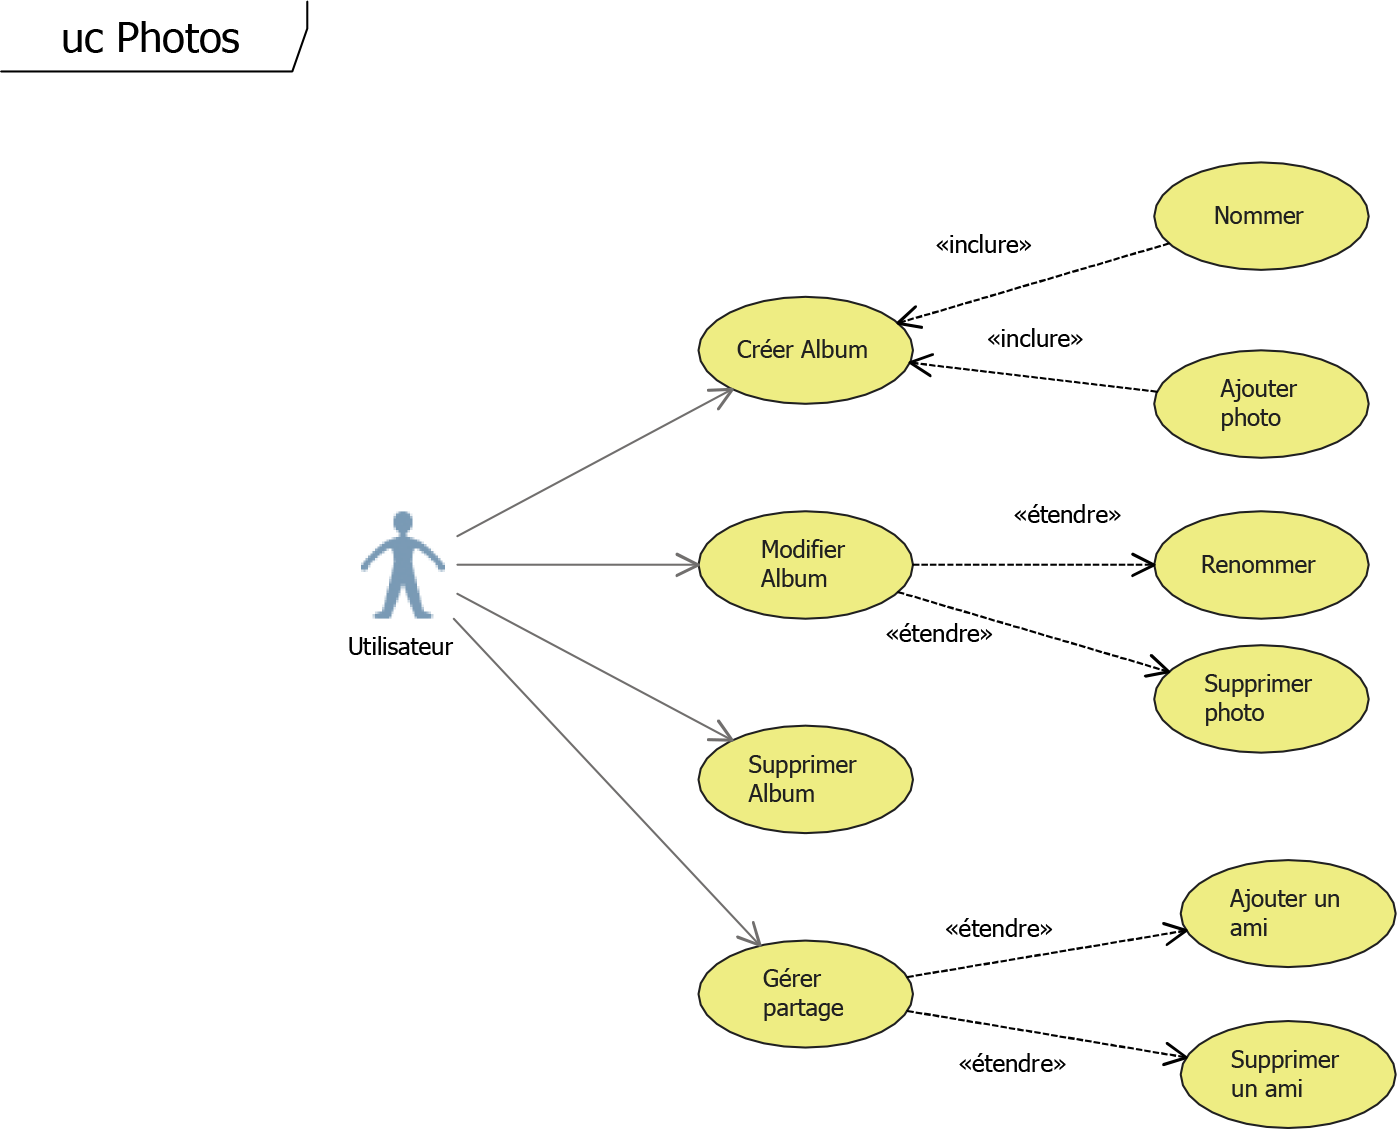
\includegraphics[scale=1]{ucPhotos.png}
        \caption{Cas d'utilisation photos}
         \label{fig:ucPhotos}
\end{figure}
\begin{figure}[!h]
        \centering 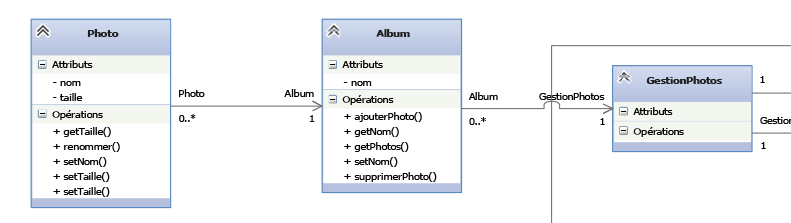
\includegraphics[scale=1]{photo.png}
        \caption{Diagramme de classe photos}
         \label{fig:photos}
\end{figure}

\newpage
\section{Modélisation de la gestion du Calendrier}
\begin{figure}[!h]
        \centering 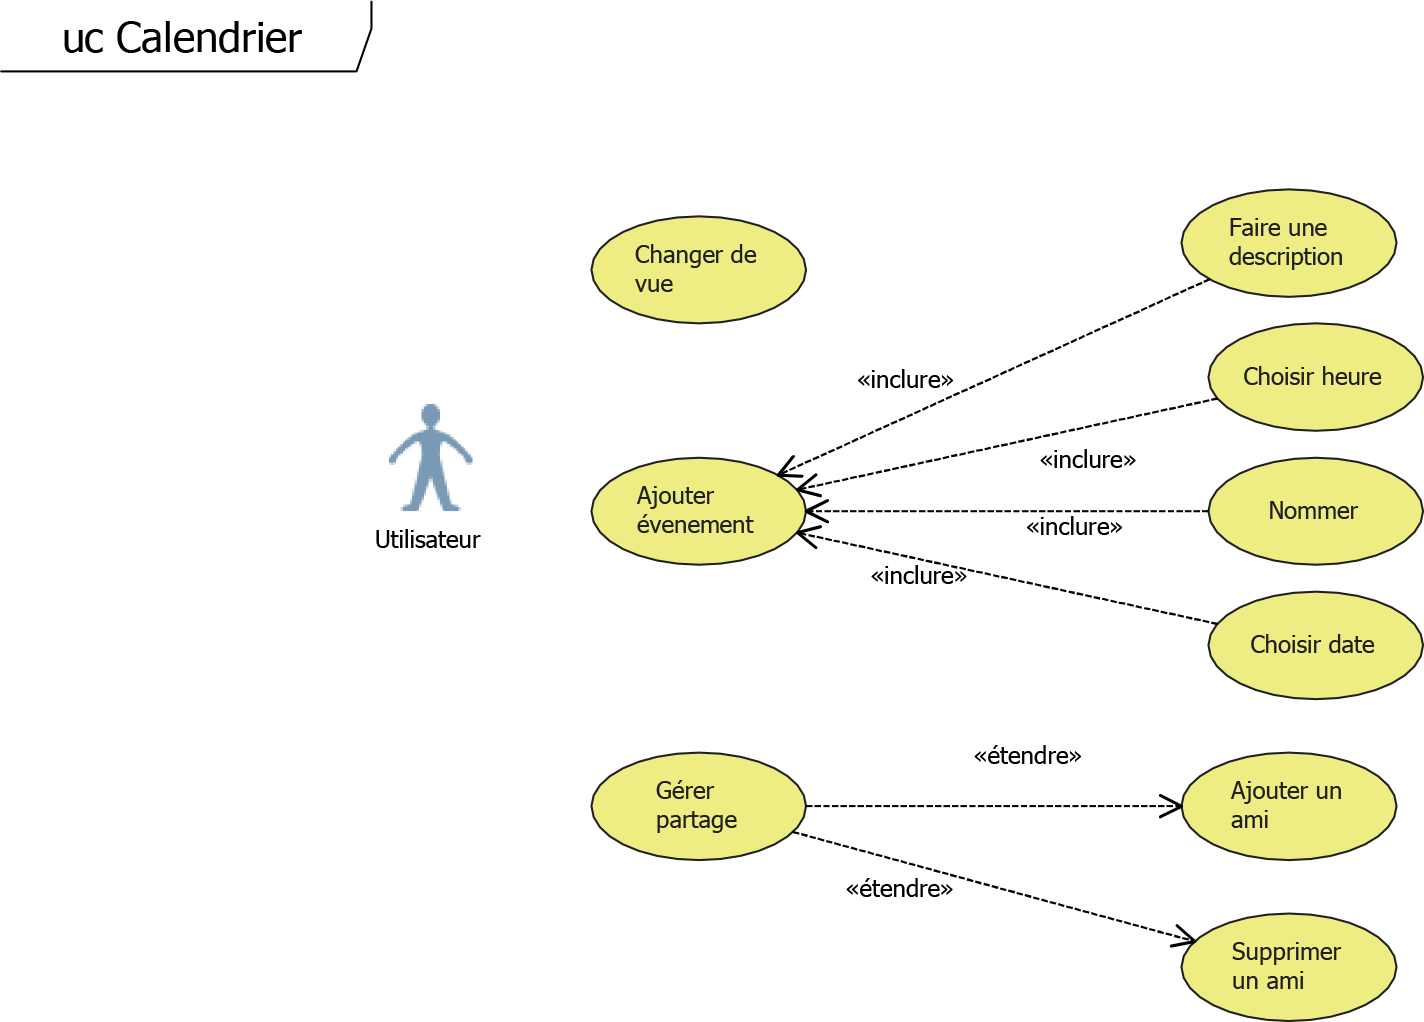
\includegraphics[scale=1]{ucCal.png}
        \caption{Cas d'utilisation calendrier}
         \label{fig:ucCal}
\end{figure}
\begin{figure}[!h]
        \centering 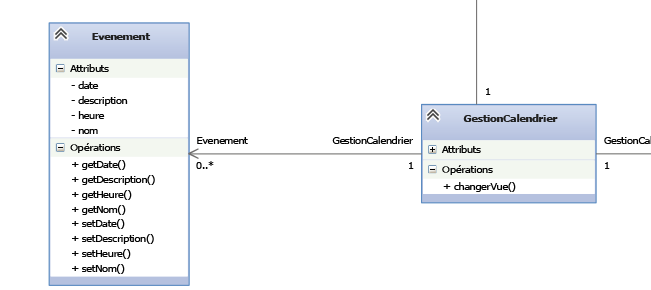
\includegraphics[scale=1]{calendrier.png}
        \caption{Diagramme de classe calendrier}
         \label{fig:cal}
\end{figure}

\newpage
\section{Modélisation de la gestion des Dépenses}
\begin{figure}[!h]
        \centering 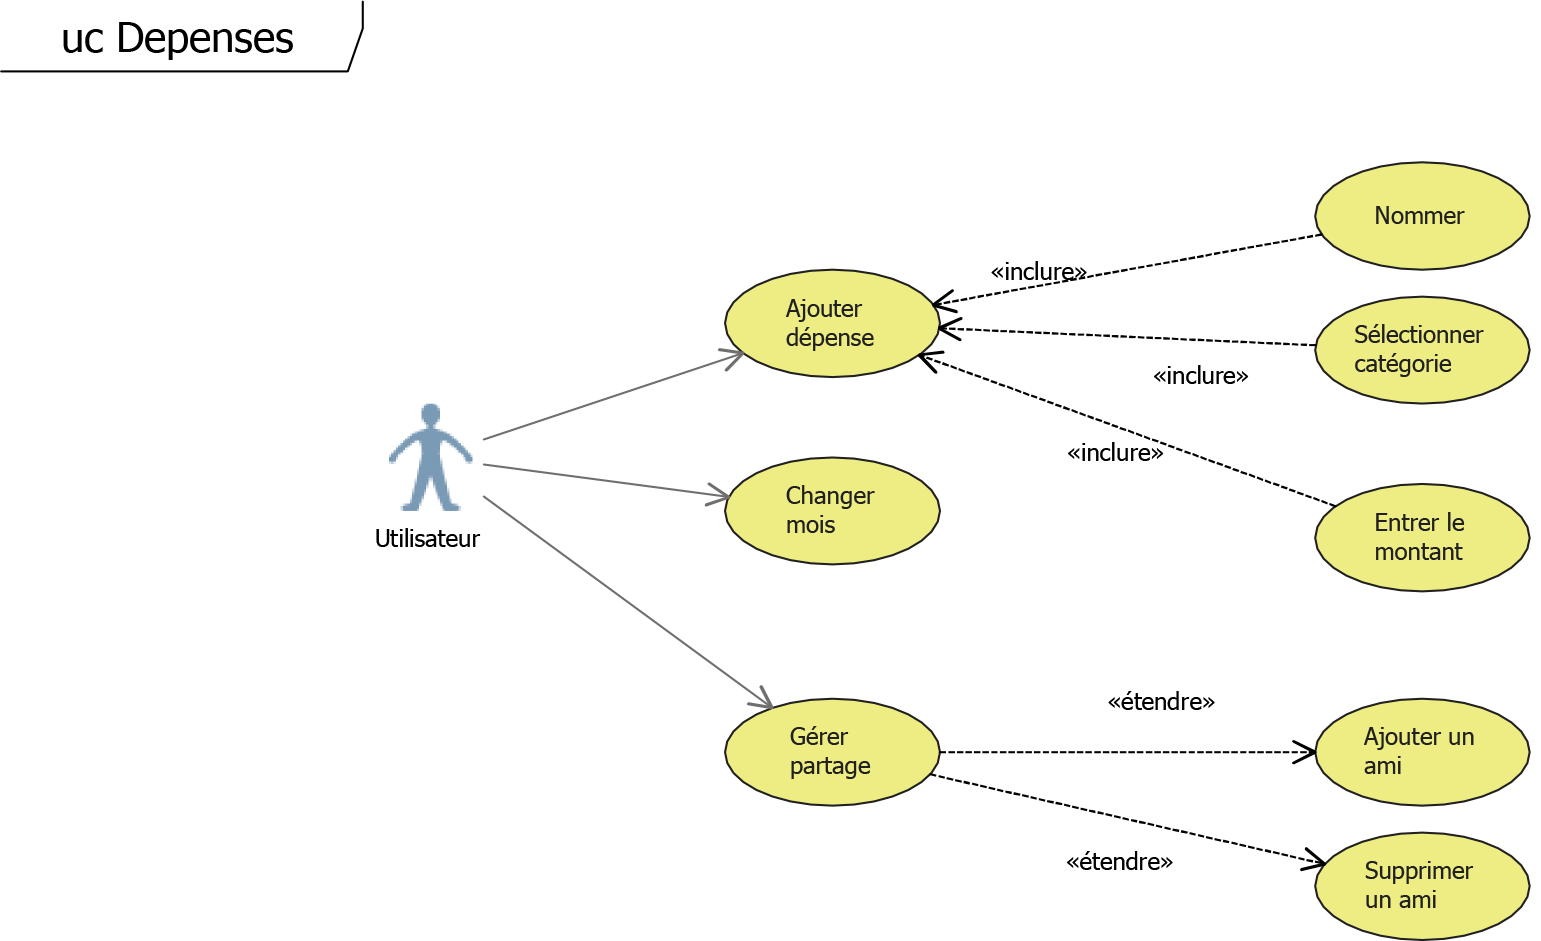
\includegraphics[scale=1]{ucDepenses.png}
        \caption{Cas d'utilisation dépenses}
         \label{fig:ucDepenses}
\end{figure}
\begin{figure}[!h]
        \centering 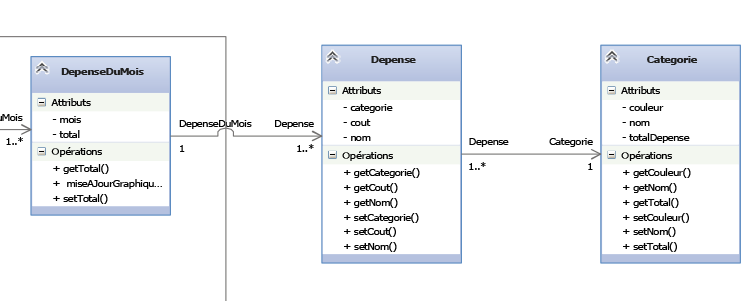
\includegraphics[scale=1]{depense.png}
        \caption{Diagramme de classe dépenses}
         \label{fig:depense}
\end{figure}!h

\newpage
\section{Modélisation de la gestion de la Carte}
\begin{figure}[!h]
        \centering 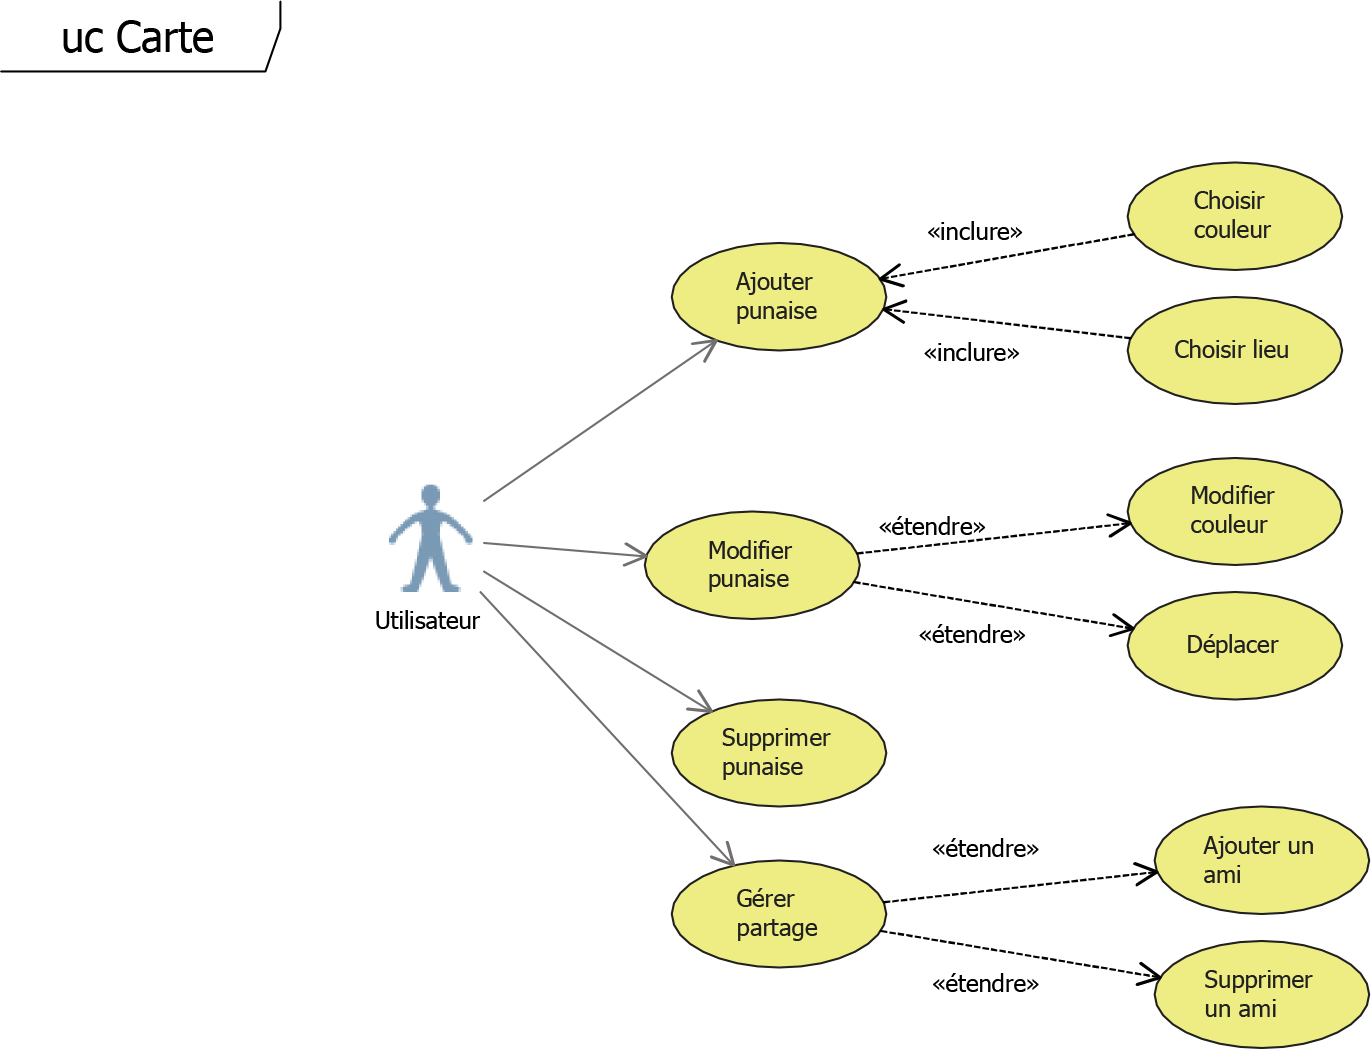
\includegraphics[scale=1]{ucCarte.png}
        \caption{Cas d'utilisation carte}
         \label{fig:ucCarte}
\end{figure}
\begin{figure}[!h]
        \centering 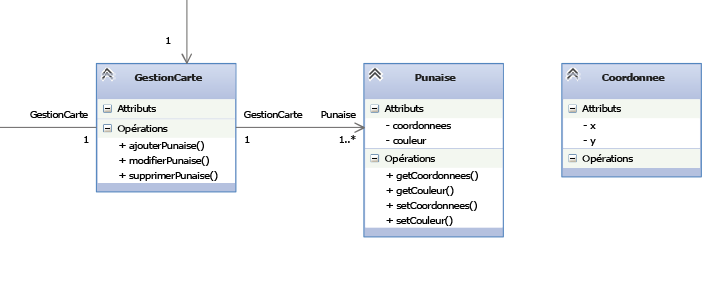
\includegraphics[scale=1]{carte.png}
        \caption{Diagramme de classe carte}
         \label{fig:carte}
\end{figure}

\newpage
\section{Modélisation de la gestion des Contacts}
\begin{figure}[!h]
        \centering 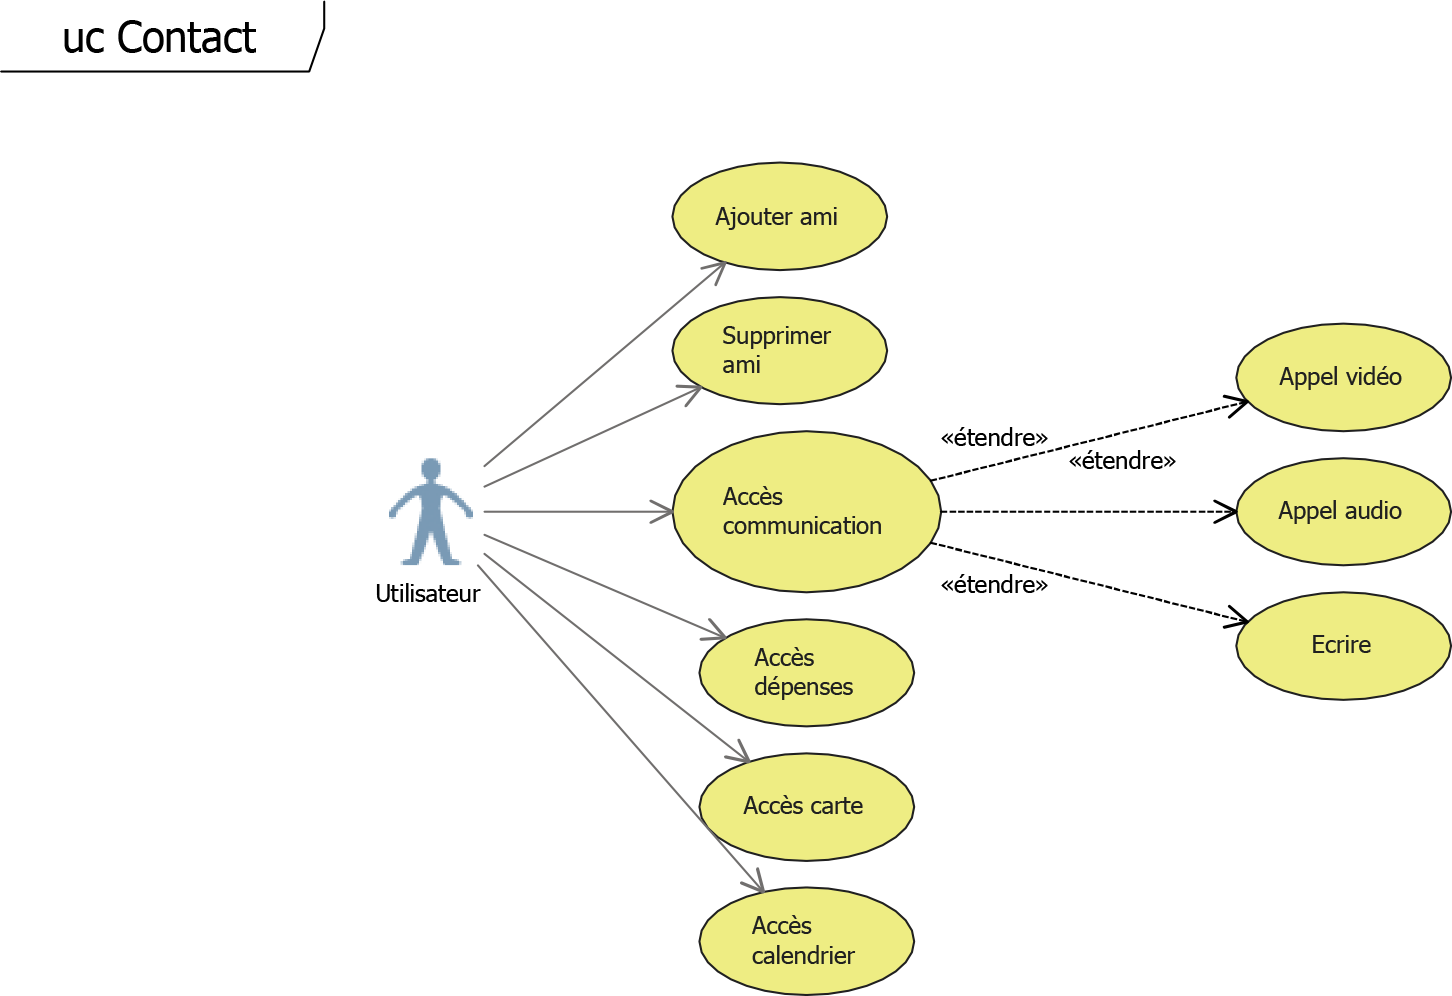
\includegraphics[scale=1]{ucContact.png}
        \caption{Cas d'utilisation contacts}
         \label{fig:ucContact}
\end{figure}
\begin{figure}[!h]
        \centering 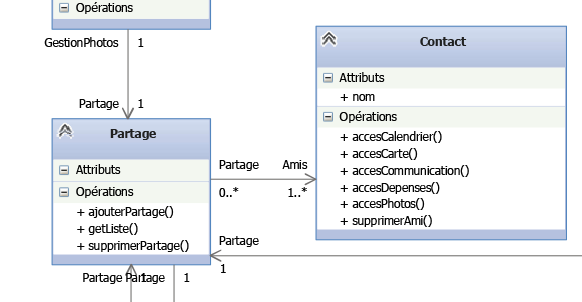
\includegraphics[scale=1]{contact.png}
        \caption{Diagramme de classe contact}
         \label{fig:contact}
\end{figure}

\newpage
\section{Diagramme de classe global}
\begin{figure}[!h]
        \centering 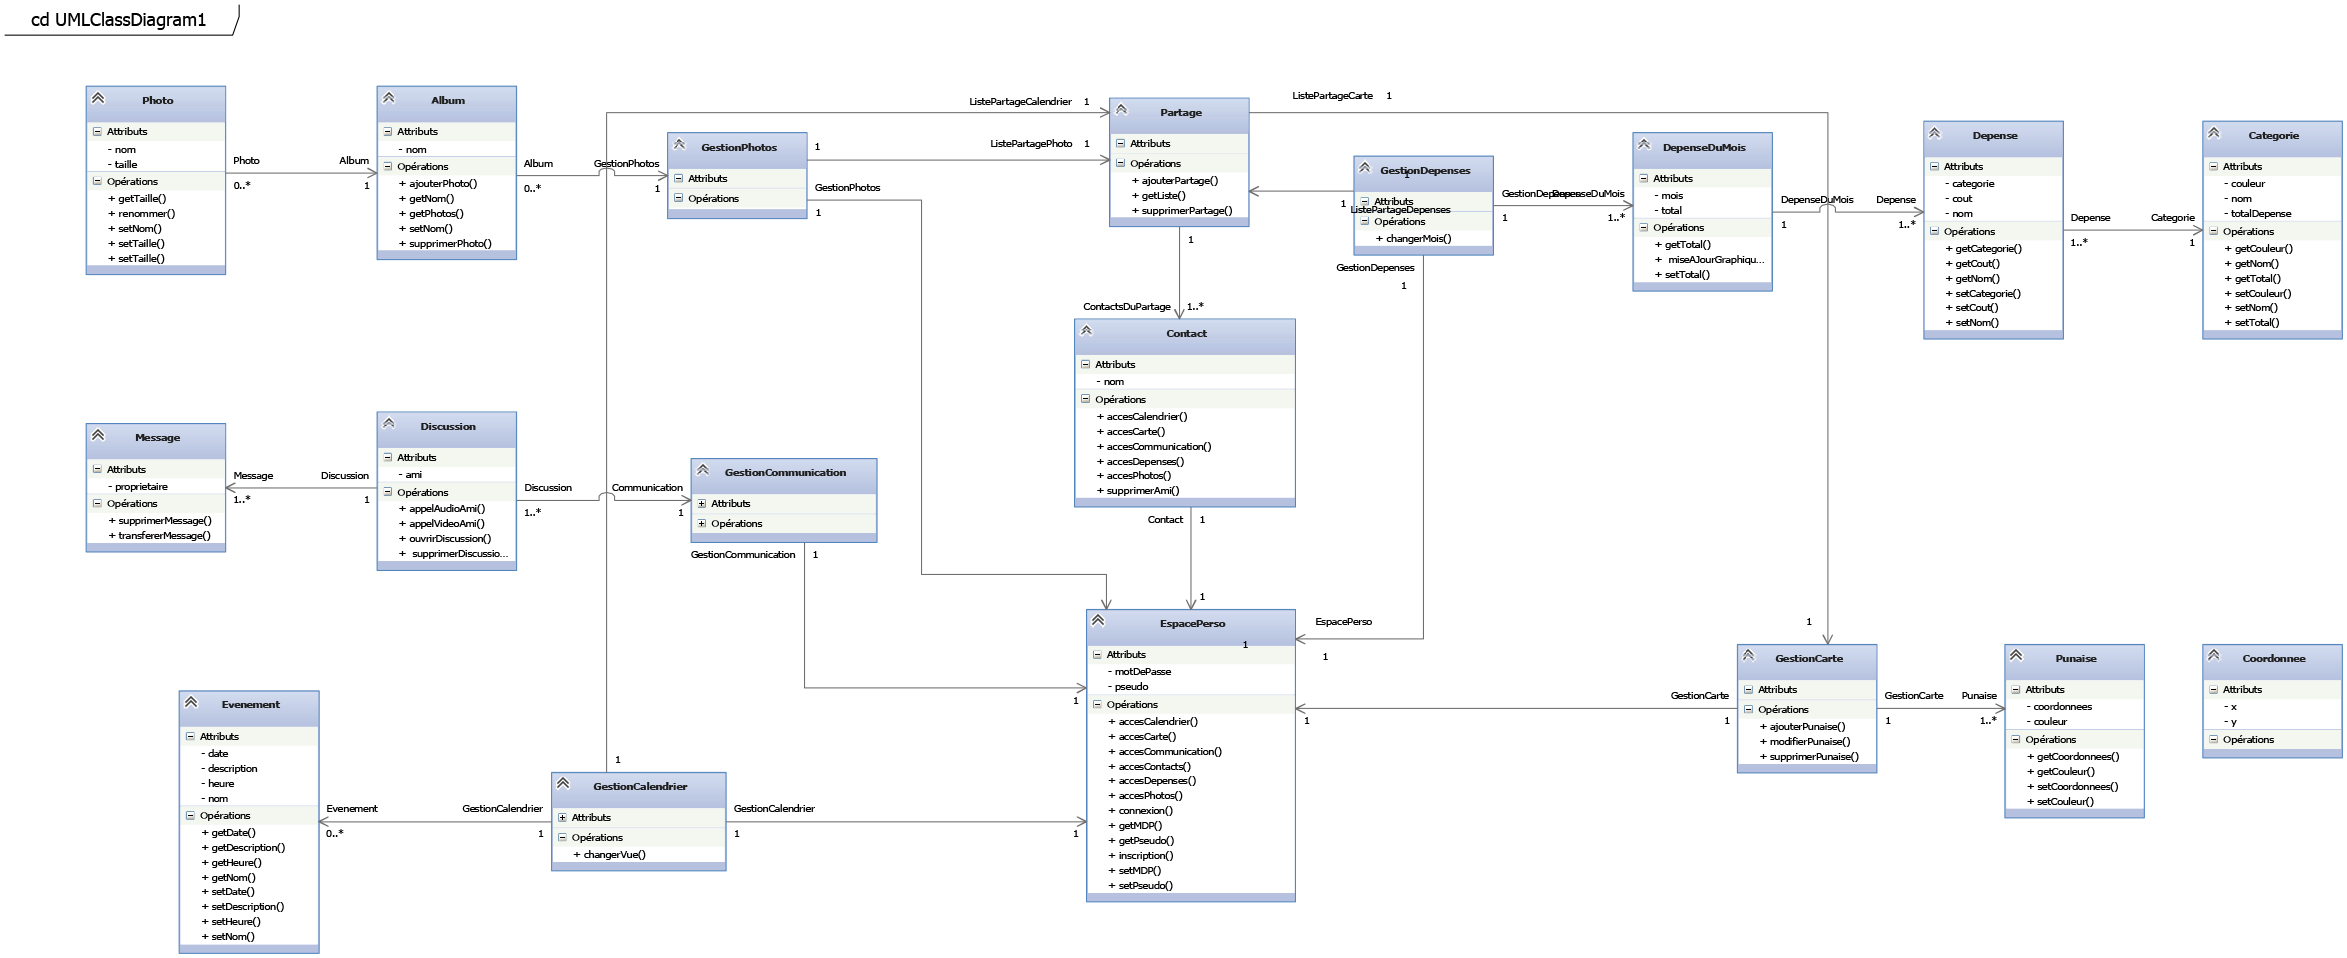
\includegraphics[scale=0.9]{classe.png}
        \caption{Diagramme de classe}
         \label{fig:classe}
\end{figure}

\begin{figure}[!h]
        \centering 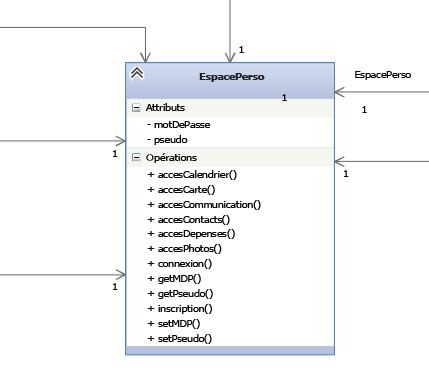
\includegraphics[scale=1]{espace.png}
        \caption{Diagramme de classe espace personnel}
         \label{fig:espace}
\end{figure}

\newpage
\section*{Conclusion \markboth{CONCLUSION}{}}
\addcontentsline{toc}{section}{Conclusion}
\newpage
\listoffigures


\end{document}